\chapter{Marco Teórico}
\section{Generalidades}
\subsection{ITS}
Los sistemas inteligentes de transporte pueden ser definidos como el matrimonio entre los avances 
en tecnologías de información y sistemas de comunicación con los vehículos y redes de caminos que 
forman parte del sistema de transporte. También pueden definirse como  la optimización de las 
funciones propias de los elementos básicos del Tránsito – Infraestructura Vial (calles y caminos) 
y Vehículos – mediante la aplicación de tecnologías avanzadas que interrelacionan tales elementos. \\

Existen dos elementos fundamentales en los Sistemas Inteligentes de Transporte  el primero es la 
capa lógica compuesta por las funciones y los procesos y el segundo es la capa física donde se 
encuentran los sistemas y las tecnologías. En ambos casos existe una coherencia con la definición 
de los servicios o aplicaciones ITS que se asocia a un marco normativo de referencia \cite{6}.
\begin{figure}[h]
    \centering
    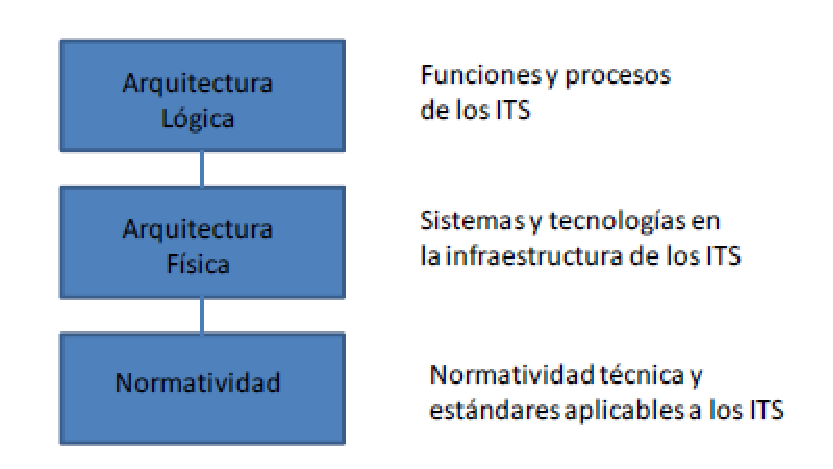
\includegraphics[width=1\textwidth]{ima/its_phpswxtBw}
    \caption{Estructura basica de los ITS. \cite{5}}
    \label{fig:mesh3}
\end{figure}
\subsection{Segmentos}
Caracterizados por su longitud, número de carriles, elemento de la red en el que comienza y elemento 
en el que finaliza. Sólo se considera un sentido de tráfico por segmento, por lo que una calle puede 
estar constituida por varios segmentos, tanto para expresar los dos sentidos de circulación (cuando 
ambos estén presentes) como las intersecciones que atraviesan \cite{7}.
\subsection{Intersecciones}
Son los elementos que principalmente definen los comienzos y finales de los segmentos, y está determinado 
por la unión de dos o más segmentos. Es aquí donde será necesario definir el derecho de paso de unos sentidos 
o direcciones respecto de otros, permitiendo realizar los cambios de dirección en el flujo de tráfico de una 
forma eficiente y segura\cite{7}.
\subsection{Flujo}
Es la cantidad de vehículos por unidad de tiempo en un determinado segmento[7].
\subsection{Velocidad}
Distancia recorrida por unidad de tiempo. La velocidad a la que circulan los vehículos es un dato importante 
para medir el nivel de congestión que existe\cite{7}.
\subsection{Tiempo}
Es el tiempo de viaje sobre un segmento del camino conocido. Esta medida es obtenida dividiendo el largo de 
la calle entre la velocidad media en recorrer la calle, en el caso de los vehículos, o en atravesarla, en el 
caso de los peatones\cite{7}.
\subsection{Ocupación}
Es el porcentaje de tiempo que en un segmento de una ruta es ocupado por vehículos\cite{7}.
\subsection{Densidad}
Es la cantidad de vehículos por unidad de distancia, en un periodo de tiempo\cite{7}.
\subsection{Funcionalidad de un semáforo}
\subsubsection{Operación constante}
Las indicaciones de rojo y verde son temporizadas a valores constantes calculados mediante el análisis del 
comportamiento histórico del tráfico en la intersección. Este tipo de operación asume que los patrones de 
tráfico pueden predecirse según sea la hora del día y, por lo tanto, no precisa de detectores de tráfico en 
la intersección que regulan. Este tipo de operación sólo suele ser utilizada cuando no se dispone de un presupuesto 
suficiente para implementar una operación flexible\cite{19}.
\subsubsection{Operación Flexible}
Las intersecciones que operan de esta manera consisten de controladores de tráfico y detectores de vehículos 
colocados en las vías próximas a la intersección. En una operación flexible se tiene que calcular la duración 
de los intervalos de verde. Los intervalos de verde pueden finalizar en una de las siguientes cuatro formas\cite{8}.
\paragraph{Alcance del tiempo máximo de tiempo verde (timing out)}
El intervalo se acaba cuando se alcanza un tiempo máximo de verde previamente establecido\cite{8}.
\paragraph{Disminución sensible del flujo de tráfico en las proximidades de la intersección (gapping out)}
Cuando se presenta un flujo ligero de tráfico que es menor que un cierto valor umbral previamente establecido\cite{8}.
\paragraph{Finalización por orden del sistema (force-off)}
Cuando un sistema de semáforos es parte de un sistema coordinado, el sistema mantiene la señal en espera con la 
operación indicada\cite{8}.
\paragraph{La señal es expulsada}
Cuando un vehículo prioritario, por ejemplo una ambulancia o un coche de bomberos, se aproxima a la intersección, 
los intervalos de verde asociados a movimientos no prioritarios deben de terminar en favor de los que están asociados 
a esos movimientos prioritarios\cite{8}.

\section{Software}
\subsection{Protocolos de comunicación enfocados al transporte}
\subsubsection{NTCIP (Estados Unidos)}
El NTCIP es un proyecto de estandarización conjunta de la AASHTO, ITE, y NEMA, Oficina del Secretario Adjunto de 
Investigación y Tecnología. NTCIP es una familia de estándares de comunicación para transmitir datos y mensajes 
entre el ordenador sistemas utilizados en los Sistemas de Transporte Inteligente (ITS). 
Un estándar de comunicaciones especifica un conjunto de reglas para los mensajes de cómo se codifican y se transmiten 
entre los dispositivos electrónicos. El equipo en cada final de una transmisión de datos utiliza la misma especificación 
para comunicarse con éxito. Es un poco como las lenguas del ser humano dado que tienen unas reglas para el alfabeto, 
vocabulario y gramática para un idioma especifico \cite{9}.
\subsubsection{SCATS (Australia)}
SCATS no requiere la intervención del operador para su funcionamiento del día a día. Sin embargo, los operadores tienen 
acceso instantáneo a la información de flujo de tráfico, estado del sistema y fallos hasta el nivel de una sola lámpara 
fundida. 
SCATS  se adapta a las exigencias de cambio de los flujos de tráfico. Por ejemplo, se puede adoptar una estrategia para 
eliminar las cargas de tráfico repentino e impredecible, tales como los cambios de clima, deportes y eventos públicos y 
conciertos.También supervisa las condiciones cambiantes de tráfico que se producen en el tráfico normal o especialmente 
cuando hay una avería, accidente u obras viales o condiciones meteorológicas adversas.Se ajusta continuamente a cambios 
de tiempo en la señal para optimizar el flujo por medición de la densidad de vehículos en cada carril \cite{10}.
\subsubsection{OCIT (Alemania)}
Significa interfaz abierta de sistemas de control de comunicación de tráfico, centro a centro. OCIT cubre las 
funciones para la comunicación entre los sistemas centrales de control de tráfico y el encaminamiento del tráfico, 
OCIT está orientado a las necesidades prácticas. Debido a los bajos costos de implementación, su uso también es adecuado 
para soluciones con presupuestos limitados \cite{11}.
\subsection{Protocolo ZIGBEE}
ZigBee es un estándar de comunicaciones inalámbricas diseñado por la ZigBee Alliance. Es un conjunto estandarizado de 
soluciones que pueden ser implementadas por cualquier fabricante. ZigBee está basado en el estándar IEEE 802.15.4 de redes 
inalámbricas de área personal (wireless  personal área Newark, WPAN) y tiene como objetivo las aplicaciones que requieren 
comunicaciones seguras con baja tasa de envío de datos y maximización de la vida útil de sus baterías\cite{12}.
\begin{figure}[h]
    \centering
    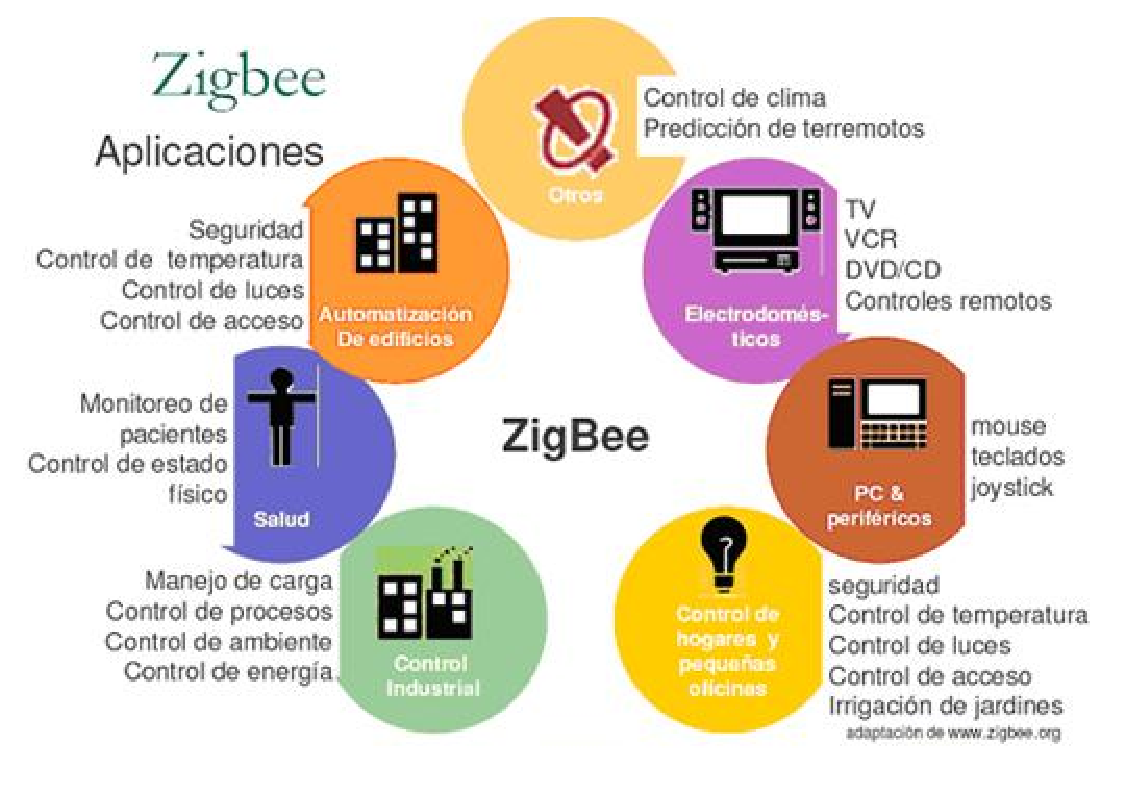
\includegraphics[width=1\textwidth]{ima/zb_phpI1D8AH}
    \caption{aplicaciones de la tecnologia ZIGBEE \cite{12}}
    \label{fig:mesh4}
\end{figure}
\section{Hardware}
\subsection{Antena GPRS}
Las siglas GPRS vienes de las palabras inglesas General Packet Radio Service( Servicio general de paquetes vía radio en 
castellano), la cual permite comunicarse vía satélite, sin necesidad de cables ni conexión física a dos terminales móviles. 
El GPRS permite pagar solo por la información enviada/recibida. Se basa en mandar la información en pequeños paquetes, es 
decir no enviar todo al mismo tiempo sino por tramas y únicamente cuando el canal estuviese libre, aprovechando así los 
huecos del mismo. Si la red está muy cargada, la trasmisión podría demorarse bastante\cite{13}.
\begin{figure}[h]
    \centering
    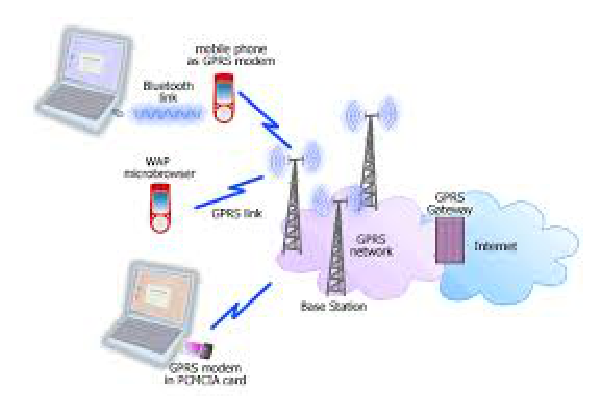
\includegraphics[width=1\textwidth]{ima/descarga_phpzcLdzH}
    \caption{Esquema de antena GPRS envío y recepción de información \cite{13}}
    \label{fig:mesh6}
\end{figure}
\subsection{Detectores de tráfico}
\subsubsection{Detectores de presión}
Consisten en una plancha de caucho en cuyo interior se sitúan dos láminas metálicas, muy cercanas entre sí, que establecen 
contacto cuando pasa un vehículo que supera un cierto peso umbral sobre la plancha. Todo este mecanismo está ubicado en la 
parte superior de una plataforma de hormigón o metálica que se empotra en el pavimento. Puede conseguirse una detección 
direccional si en vez de las dos láminas se ponen cuatro, enfrentadas dos a dos \cite{14}.
\subsubsection{Detectores magnéticos}
Detectan la distorsión del campo magnético producida por el paso sobre ellos de una masa metálica. Están formados por un 
tubo metálico en cuyo interior hay un núcleo de hierro con una bobina conectada a un amplificador. Los detectores más 
habituales que emplean esta tecnología no son capaces de detectar la dirección del movimiento, por lo que se fueron 
incorporando mejoras en su diseño dando lugar a los llamados detectores magnéticos compensados, formados por cuatro 
núcleos, que permiten distinguir el sentido de la marcha de la masa metálica que circula sobre ellos\cite{14}.
\subsubsection{Detectores de lazo}
Constituyen el tipo de detector más utilizado en las vías públicas actuales. Su principio de funcionamiento se basa en emplear 
las características de un lazo magnético situado sobre la superficie de la carretera y las fluctuaciones eléctricas producidas 
por la aproximación de un objeto metálico (que en este caso es un vehículo) para detectar su presencia y su paso. 

Efectivamente, mientras circula una corriente alterna por el lazo metálico situado sobre la carretera, se crea un campo magnético 
de la misma frecuencia cerca de la superficie de la carretera. Si un objeto metálico entra en este campo magnético, entonces la 
inducción magnética causa corrientes sobre el objeto metálico y como resultado se produce una variación en la impedancia a la 
salida del lazo magnético. Cuando se detecta un cambio de impedancia se detecta un vehículo. El cambio de inductancia provocado 
por el paso de vehículos varía según el tipo de vehículo. Este tipo de detectores son más sensitivos a vehículos pequeños que a 
vehículos de gran volumen. Entre las medidas que este tipo de detector de tráfico puede proporcionar destacan las siguientes:
\begin{itemize}
    \item Presencia de un vehículo.
    \item Tipo de vehículo (mediante el empleo de técnicas de reconocimiento de patrones es posible diferenciar entre seis o más tipos de vehículos).
    \item Velocidad del vehículo (mediante el uso de lazos dobles).
    \item Ocupación de los lazos.
    \item Intervalo de tiempo entre vehículos.
\end{itemize}

\subsubsection{Detectores de Radar.}
Constan de un aparato emisor y otro receptor de ondas electromagnéticas y generalmente se suspenden sobre la vía o se colocan 
lateralmente a ella. En la actualidad se emplean dos tipos de detectores de radar de microondas en las aplicaciones de 
gestión del tráfico. 
El primero transmite energía electromagnética a una frecuencia constante midiendo la velocidad de los vehículos dentro de su 
campo de visión usando el principio Dopler, en el que la diferencia de frecuencia entre las señales transmitidas y recibidas 
es proporcional a la velocidad del vehículo. Por lo tanto, la detección de una variación en la frecuencia denota el paso de un vehículo. 
Este tipo de sensor no puede detectar vehículos parados y, por lo tanto, no es adecuado para aplicaciones que precisan detectar 
la presencia de vehículos tales como regulación de semáforos o líneas de parada obligatoria. 
El segundo tipo de detector de radar de microondas transmite una onda en forma de diente de sierra, también denominada onda continua 
modulada en frecuencia, que varía la frecuencia transmitida de forma continua en el tiempo. Los vehículos parados se detectan midiendo 
el rango desde el detector hasta el vehículo y también calculando la velocidad del vehículo midiendo el tiempo que le lleva al vehículo 
viajar entre dos marcas internas que representan distancias conocidas para el radar. Al disponer de la característica de detección de 
vehículos parados, este detector suele denomina se radar de microondas de presencia real\cite{14}.
\subsubsection{Detector pasivo de infrarrojo}
Este tipo de dispositivo es capaz de detectar el paso y la presencia de vehículos, pero no su velocidad. 
Su método de funcionamiento se basa en un detector sensitivo a la energía de fotones colocado en un plano focal para medir la energía 
infrarroja emitida por los objetos en el campo de visión del detector. Los detectores pasivos no transmiten energía por si mismos. 
Cuando un vehículo entra en la zona de detección produce un cambio en la energía medida normalmente desde la superficie de la vía en 
la ausencia de vehículos. El cambio en la energía es proporcional a la temperatura absoluta del vehículo y la emisividad de la 
superficie metálica del vehículo (la emisividad es el cociente de la energía emitida respecto al radiante perfecto de energía a la misma 
temperatura). 
La diferencia de energía que es capaz de detectar este detector se reduce ante condiciones meteorológicas adversas 
(lluvia, nieve, niebla,...)\cite{14}.
\subsubsection{ Detector activo de infrarrojo}
Su funcionamiento es similar al de los detectores de radar por microondas. Los más comunes utilizan un diodo láser para emitir energía 
en el espectro cercano al infrarrojo, una porción del cual vuelve al receptor del detector desde el vehículo de su campo de visión. 
Los detectores basados en el radar láser pueden suministrar la presencia, el paso y la velocidad de vehículos. 
La medición de la velocidad se realiza anotando el tiempo que le lleva a un vehículo cruzar dos haces de infrarrojos que están ubicados 
a una distancia conocida. Algunos de estos detectores son capaces de clasificar los vehículos contrastando las mediciones con unos 
ficheros modelos \cite{14}.
\subsubsection{Detectores de ultrasonido}
Los detectores ultrasónicos emiten sonidos a una frecuencia entre los 25 kHz a los 50 kHz (según sea el fabricante). 
Estas frecuencias no están en la franja audible. Una porción de la energía transmitida se refleja desde la carretera o la superficie 
del vehículo de nuevo al detector y se procesa para dar el paso y presencia de vehículos. Un detector típico de presencia ultrasónico 
emite energía ultrasónica en forma de pulsos. El tiempo que le lleva al pulso dejar el detector, chocar contra la superficie y regresar 
al detector es proporcional al rango del detector a la superficie. Cuando un vehículo se introduce en su campo de visión se mide el rango 
desde el detector hasta el vehículo, obteniéndose un rango menor que el producido sobre la vía lo que produce en el detector una señal 
de detección de vehículo \cite{14}.
\subsubsection{ Detectores acústicos pasivos}
El tráfico de vehículos produce una energía acústica o sonido audible desde una variedad de fuentes dentro del vehículo y desde la 
interacción de los neumáticos del vehículo con la superficie de la vía. Cuando un vehículo pasa por la zona de detección, el algoritmo 
de procesado de señales detecta un incremento respecto a la energía del sonido y se genera una señal de presencia de vehículo. 
Cuando el vehículo abandona la zona de detección, la energía del sonido decrece hasta por debajo de un nivel de detección umbral 
terminando la señal de presencia de vehículo\cite{14}.
\subsubsection{Procesadores de imágenes de video}
Estos detectores identifican los vehículos y sus parámetros de flujo de tráfico asociados mediante el análisis de las imágenes 
suministradas por cámaras de vídeo. Estas imágenes se digitalizan y se analizan para identificar los cambios observables entre 
imágenes sucesivas, es decir, los cambios de los niveles de contraste entre píxeles adyacentes. Por lo tanto estos detectores 
pueden suministrar información sobre el paso, presencia, velocidad, longitud y cambios de carriles de vehículos según sea el 
tipo de técnica de procesado de imágenes utilizada\cite{14}.
\begin{figure}[h]
    \centering
    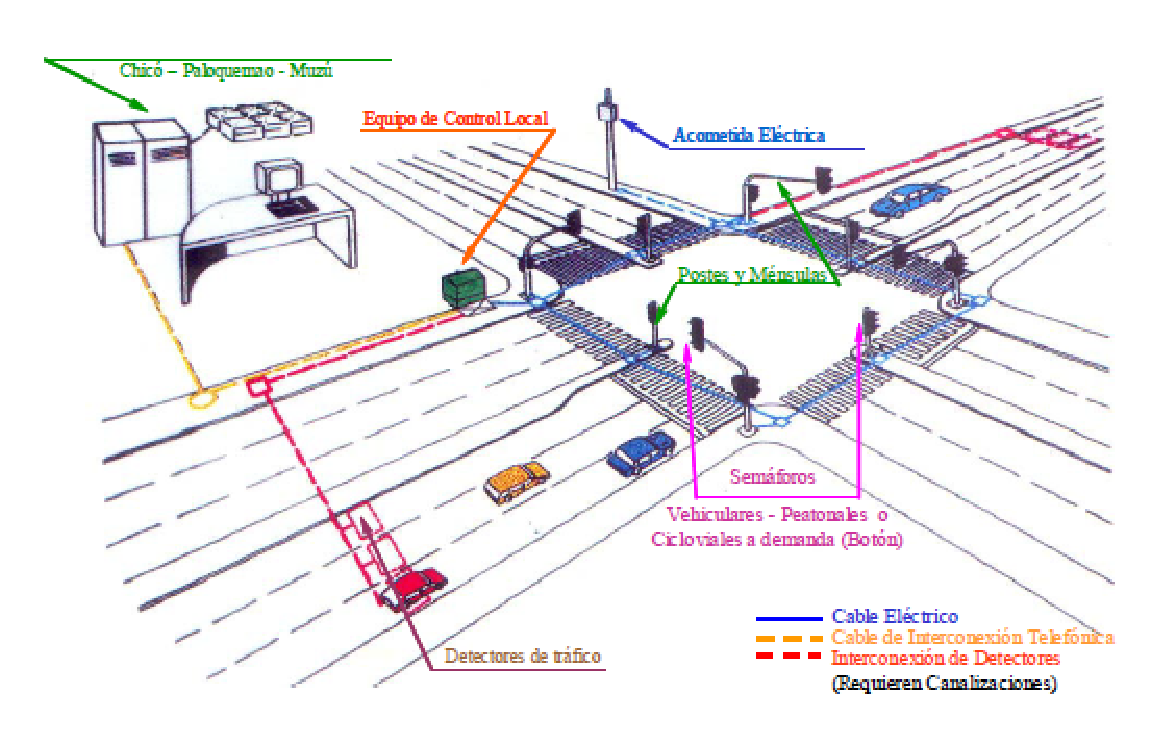
\includegraphics[width=1\textwidth]{ima/ca_phpB1BaNG}
    \caption{Configuración  típica de gestión de tráfico. Conexión del centro de control con una inetrsección semaforizada para Bogotá D.C. \cite{5}}
    \label{fig:mesh5}
\end{figure}